\documentclass[]{article}
\usepackage{lmodern}
\usepackage{amssymb,amsmath}
\usepackage{ifxetex,ifluatex}
\usepackage{fixltx2e} % provides \textsubscript
\ifnum 0\ifxetex 1\fi\ifluatex 1\fi=0 % if pdftex
  \usepackage[T1]{fontenc}
  \usepackage[utf8]{inputenc}
\else % if luatex or xelatex
  \ifxetex
    \usepackage{mathspec}
  \else
    \usepackage{fontspec}
  \fi
  \defaultfontfeatures{Ligatures=TeX,Scale=MatchLowercase}
\fi
% use upquote if available, for straight quotes in verbatim environments
\IfFileExists{upquote.sty}{\usepackage{upquote}}{}
% use microtype if available
\IfFileExists{microtype.sty}{%
\usepackage{microtype}
\UseMicrotypeSet[protrusion]{basicmath} % disable protrusion for tt fonts
}{}
\usepackage[margin=1in]{geometry}
\usepackage{hyperref}
\hypersetup{unicode=true,
            pdftitle={Dimensionality reduction},
            pdfauthor={Lukas Forst},
            pdfborder={0 0 0},
            breaklinks=true}
\urlstyle{same}  % don't use monospace font for urls
\usepackage{color}
\usepackage{fancyvrb}
\newcommand{\VerbBar}{|}
\newcommand{\VERB}{\Verb[commandchars=\\\{\}]}
\DefineVerbatimEnvironment{Highlighting}{Verbatim}{commandchars=\\\{\}}
% Add ',fontsize=\small' for more characters per line
\usepackage{framed}
\definecolor{shadecolor}{RGB}{248,248,248}
\newenvironment{Shaded}{\begin{snugshade}}{\end{snugshade}}
\newcommand{\AlertTok}[1]{\textcolor[rgb]{0.94,0.16,0.16}{#1}}
\newcommand{\AnnotationTok}[1]{\textcolor[rgb]{0.56,0.35,0.01}{\textbf{\textit{#1}}}}
\newcommand{\AttributeTok}[1]{\textcolor[rgb]{0.77,0.63,0.00}{#1}}
\newcommand{\BaseNTok}[1]{\textcolor[rgb]{0.00,0.00,0.81}{#1}}
\newcommand{\BuiltInTok}[1]{#1}
\newcommand{\CharTok}[1]{\textcolor[rgb]{0.31,0.60,0.02}{#1}}
\newcommand{\CommentTok}[1]{\textcolor[rgb]{0.56,0.35,0.01}{\textit{#1}}}
\newcommand{\CommentVarTok}[1]{\textcolor[rgb]{0.56,0.35,0.01}{\textbf{\textit{#1}}}}
\newcommand{\ConstantTok}[1]{\textcolor[rgb]{0.00,0.00,0.00}{#1}}
\newcommand{\ControlFlowTok}[1]{\textcolor[rgb]{0.13,0.29,0.53}{\textbf{#1}}}
\newcommand{\DataTypeTok}[1]{\textcolor[rgb]{0.13,0.29,0.53}{#1}}
\newcommand{\DecValTok}[1]{\textcolor[rgb]{0.00,0.00,0.81}{#1}}
\newcommand{\DocumentationTok}[1]{\textcolor[rgb]{0.56,0.35,0.01}{\textbf{\textit{#1}}}}
\newcommand{\ErrorTok}[1]{\textcolor[rgb]{0.64,0.00,0.00}{\textbf{#1}}}
\newcommand{\ExtensionTok}[1]{#1}
\newcommand{\FloatTok}[1]{\textcolor[rgb]{0.00,0.00,0.81}{#1}}
\newcommand{\FunctionTok}[1]{\textcolor[rgb]{0.00,0.00,0.00}{#1}}
\newcommand{\ImportTok}[1]{#1}
\newcommand{\InformationTok}[1]{\textcolor[rgb]{0.56,0.35,0.01}{\textbf{\textit{#1}}}}
\newcommand{\KeywordTok}[1]{\textcolor[rgb]{0.13,0.29,0.53}{\textbf{#1}}}
\newcommand{\NormalTok}[1]{#1}
\newcommand{\OperatorTok}[1]{\textcolor[rgb]{0.81,0.36,0.00}{\textbf{#1}}}
\newcommand{\OtherTok}[1]{\textcolor[rgb]{0.56,0.35,0.01}{#1}}
\newcommand{\PreprocessorTok}[1]{\textcolor[rgb]{0.56,0.35,0.01}{\textit{#1}}}
\newcommand{\RegionMarkerTok}[1]{#1}
\newcommand{\SpecialCharTok}[1]{\textcolor[rgb]{0.00,0.00,0.00}{#1}}
\newcommand{\SpecialStringTok}[1]{\textcolor[rgb]{0.31,0.60,0.02}{#1}}
\newcommand{\StringTok}[1]{\textcolor[rgb]{0.31,0.60,0.02}{#1}}
\newcommand{\VariableTok}[1]{\textcolor[rgb]{0.00,0.00,0.00}{#1}}
\newcommand{\VerbatimStringTok}[1]{\textcolor[rgb]{0.31,0.60,0.02}{#1}}
\newcommand{\WarningTok}[1]{\textcolor[rgb]{0.56,0.35,0.01}{\textbf{\textit{#1}}}}
\usepackage{graphicx,grffile}
\makeatletter
\def\maxwidth{\ifdim\Gin@nat@width>\linewidth\linewidth\else\Gin@nat@width\fi}
\def\maxheight{\ifdim\Gin@nat@height>\textheight\textheight\else\Gin@nat@height\fi}
\makeatother
% Scale images if necessary, so that they will not overflow the page
% margins by default, and it is still possible to overwrite the defaults
% using explicit options in \includegraphics[width, height, ...]{}
\setkeys{Gin}{width=\maxwidth,height=\maxheight,keepaspectratio}
\IfFileExists{parskip.sty}{%
\usepackage{parskip}
}{% else
\setlength{\parindent}{0pt}
\setlength{\parskip}{6pt plus 2pt minus 1pt}
}
\setlength{\emergencystretch}{3em}  % prevent overfull lines
\providecommand{\tightlist}{%
  \setlength{\itemsep}{0pt}\setlength{\parskip}{0pt}}
\setcounter{secnumdepth}{0}
% Redefines (sub)paragraphs to behave more like sections
\ifx\paragraph\undefined\else
\let\oldparagraph\paragraph
\renewcommand{\paragraph}[1]{\oldparagraph{#1}\mbox{}}
\fi
\ifx\subparagraph\undefined\else
\let\oldsubparagraph\subparagraph
\renewcommand{\subparagraph}[1]{\oldsubparagraph{#1}\mbox{}}
\fi

%%% Use protect on footnotes to avoid problems with footnotes in titles
\let\rmarkdownfootnote\footnote%
\def\footnote{\protect\rmarkdownfootnote}

%%% Change title format to be more compact
\usepackage{titling}

% Create subtitle command for use in maketitle
\providecommand{\subtitle}[1]{
  \posttitle{
    \begin{center}\large#1\end{center}
    }
}

\setlength{\droptitle}{-2em}

  \title{Dimensionality reduction}
    \pretitle{\vspace{\droptitle}\centering\huge}
  \posttitle{\par}
    \author{Lukas Forst}
    \preauthor{\centering\large\emph}
  \postauthor{\par}
      \predate{\centering\large\emph}
  \postdate{\par}
    \date{17 listopadu 2019}


\begin{document}
\maketitle

\hypertarget{introduction}{%
\subsection{Introduction}\label{introduction}}

The goal of this tutorial is to get familiar with some basic methods for
dimensionality reduction, complete you own implementation of the
\textbf{Isomap algorithm} (in cooperation with \emph{Multidimensional
scaling}), experiment with its parameters and compare with other
techniques of dimensionality reduction (\textbf{PCA}, \textbf{t-SNE}).

\hypertarget{background}{%
\subsection{Background}\label{background}}

The data you will be working with are vector representations of words in
a latent (unknown) high-dimensional space. This representation of words,
also know as word embedding, differs from standard bag-of-words (BoW,
TFIDF, etc.) representations in that the meaning of the words is
distributed across all the dimensions. Generally speaking, the word
embedding algorithms seek to learn a mapping projecting the original BoW
representation (simple word index into a given vocabulary) into a
lower-dimensional (but still too high for our cause) continuous
vector-space, based on their distributional properties observed in some
raw text corpus. This distributional semantics approach to word
representations is based on the basic idea that linguistic items with
similar distributions typically have similar meanings, i.e.~words that
often appear in a similar context (words that surround them) tend to
have similar (vector) representations.

Speciffically, the data you are presented with are vector
representations coming from the most popular algorithm for word
embedding known as word2vec\footnote{Tomas Mikolov, Ilya Sutskever, Kai
  Chen, Greg S Corrado, and Jeff Dean. Distributed representations of
  words and phrases and their compositionality. In \emph{Advances in
  neural information processing systems}, pages 3111-3119, 2013.} by
Tomas Mikolov (VUT-Brno alumni). \emph{Word2vec} is a (shallow) neural
model learning the projection of BoW word representations into a latent
space by the means of gradient descend. Your task is to further reduce
the dimensionality of the word representations to get a visual insight
into what has been learned.

\hypertarget{data}{%
\subsection{Data}\label{data}}

You are given 300-dimensional word2vec vector embeddings in the file
\emph{data.csv} with corresponding word labels in \emph{labels.txt} for
each line. Each of these words comes from one of 10 selected classes of
synonyms, which can be recognized (and depicted) w.r.t. labels denoted
in the file \emph{colors.csv}

\hypertarget{tasks}{%
\subsection{Tasks}\label{tasks}}

\begin{enumerate}
\def\labelenumi{\arabic{enumi}.}
\tightlist
\item
  \textbf{Load the dataset of 165 words}, each represented as a
  300-dimensional vector. Each word is assigned to one of 10 clusters.
\end{enumerate}

\begin{Shaded}
\begin{Highlighting}[]
\CommentTok{\#Load the dataset of 165 words}
\NormalTok{mydata <{-}}\StringTok{ }\KeywordTok{read.csv}\NormalTok{(}\StringTok{\textquotesingle{}data.csv\textquotesingle{}}\NormalTok{, }\DataTypeTok{header =} \OtherTok{FALSE}\NormalTok{)}
\NormalTok{mylabels <{-}}\StringTok{ }\KeywordTok{read.csv}\NormalTok{(}\StringTok{\textquotesingle{}labels.txt\textquotesingle{}}\NormalTok{, }\DataTypeTok{header =} \OtherTok{FALSE}\NormalTok{)}
\NormalTok{mycolors <{-}}\StringTok{ }\KeywordTok{read.csv}\NormalTok{(}\StringTok{\textquotesingle{}colors.csv\textquotesingle{}}\NormalTok{, }\DataTypeTok{header =} \OtherTok{FALSE}\NormalTok{)}
\end{Highlighting}
\end{Shaded}

The data is in the matrix \texttt{mydata}, cluster assignment in
\texttt{mycolors} and the actual words (useful for visualization) in
\texttt{mylabels}. You can plot the data by using only the first 2
dimensions.

\begin{Shaded}
\begin{Highlighting}[]
\KeywordTok{PlotPoints}\NormalTok{(mydata[,}\KeywordTok{c}\NormalTok{(}\DecValTok{1}\NormalTok{,}\DecValTok{2}\NormalTok{)], mylabels, mycolors)}
\end{Highlighting}
\end{Shaded}

\begin{verbatim}
## deldir 0.1-23
\end{verbatim}

\begin{verbatim}
## 
##      PLEASE NOTE:  The components "delsgs" and "summary" of the
##  object returned by deldir() are now DATA FRAMES rather than
##  matrices (as they were prior to release 0.0-18).
##  See help("deldir").
##  
##      PLEASE NOTE: The process that deldir() uses for determining
##  duplicated points has changed from that used in version
##  0.0-9 of this package (and previously). See help("deldir").
\end{verbatim}

\includegraphics{dimensionality_reduction_files/figure-latex/unnamed-chunk-3-1.pdf}

\begin{enumerate}
\def\labelenumi{\arabic{enumi}.}
\setcounter{enumi}{1}
\tightlist
\item
  \textbf{Implement ISO-MAP dimensionality reduction procedure}.
\end{enumerate}

\begin{itemize}
\tightlist
\item
  Use \emph{k}-NN method to construct the neighborhood graph (sparse
  matrix).

  \begin{itemize}
  \tightlist
  \item
    For simplicity, you can use \texttt{get.knn} method available in
    \texttt{FNN} package.
  \end{itemize}
\item
  Compute shortest-paths (geodesic) matrix using your favourite
  algorithm.

  \begin{itemize}
  \tightlist
  \item
    Tip: Floyd-Warshall algorithm can be implemented easily here.
  \end{itemize}
\item
  Project the geodesic distance matrix into 2D space with (Classical)
  Multidimensional Scaling (\texttt{cmdscale} functions in R).
\item
  Challenge: you may simply use PCA to do the same, but be careful to
  account for a proper normalization (centering) of the geodesic
  (kernel) matrix (see Kernel PCA for details).
\end{itemize}

An expected result (for \emph{k} = 5) should look similar (not
necessarily exactly the same) to following
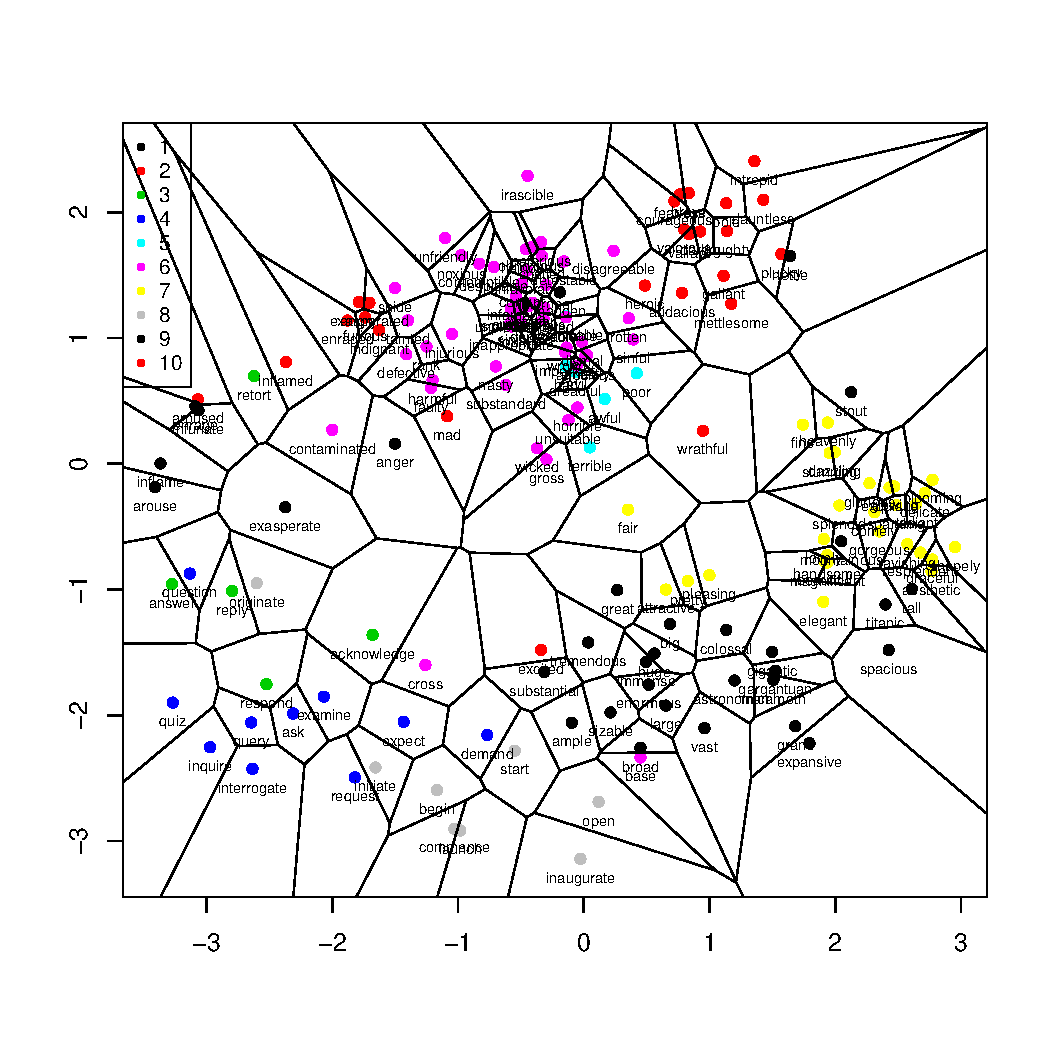
\includegraphics{graph_iso.pdf}

\begin{Shaded}
\begin{Highlighting}[]
\CommentTok{\#ADD YOUR CODE HERE!}
\CommentTok{\#REMOVE eval=FALSE arguments}

\CommentTok{\#1.Determine the neighbors of each point (k{-}NN)}

\CommentTok{\#2.Construct a neighborhood graph.}
\CommentTok{\#Each point is connected to other if it is a K nearest neighbor.}
\CommentTok{\#Edge length equal to Euclidean distance.}

\CommentTok{\#3.Compute shortest path between two nodes. (Floyd{-}Warshall algorithm)}

\CommentTok{\#4.(classical) multidimensional scaling}
\NormalTok{fit <{-}}\StringTok{ }\KeywordTok{cmdscale}\NormalTok{(D,}\DataTypeTok{eig=}\OtherTok{TRUE}\NormalTok{, }\DataTypeTok{k=}\DecValTok{2}\NormalTok{)}
\KeywordTok{PlotPoints}\NormalTok{(fit}\OperatorTok{$}\NormalTok{points, mylabels, mycolors)}
\end{Highlighting}
\end{Shaded}

\begin{enumerate}
\def\labelenumi{\arabic{enumi}.}
\setcounter{enumi}{2}
\tightlist
\item
  \textbf{Visually compare PCA, ISOMAP and t-SNE} by plotting the
  word2vec data, embedded into 2D using the \texttt{Plotpoints}
  function. Try finding the optimal \emph{k} value for ISOMAP's nearest
  neighbour.
\end{enumerate}

\begin{Shaded}
\begin{Highlighting}[]
\CommentTok{\#Principal component analysis}
\NormalTok{fitPCA <{-}}\StringTok{ }\KeywordTok{prcomp}\NormalTok{(mydata, }\DataTypeTok{center =} \OtherTok{TRUE}\NormalTok{, }\DataTypeTok{scale. =} \OtherTok{TRUE}\NormalTok{)}
\KeywordTok{PlotPoints}\NormalTok{(fitPCA}\OperatorTok{$}\NormalTok{x[,}\KeywordTok{c}\NormalTok{(}\DecValTok{1}\NormalTok{,}\DecValTok{2}\NormalTok{)], mylabels, mycolors)}

\CommentTok{\#t{-}SNE (T{-}Distributed Stochastic Neighbor Embedding)}
\CommentTok{\#install.packages(\textquotesingle{}tsne\textquotesingle{})}
\KeywordTok{library}\NormalTok{(tsne)}
\NormalTok{fittsne <{-}}\StringTok{ }\KeywordTok{tsne}\NormalTok{(mydata, }\DataTypeTok{k =} \DecValTok{2}\NormalTok{)}
\KeywordTok{PlotPoints}\NormalTok{(fittsne, mylabels, mycolors)}
\end{Highlighting}
\end{Shaded}

\begin{enumerate}
\def\labelenumi{\arabic{enumi}.}
\setcounter{enumi}{3}
\tightlist
\item
  \textbf{Observe the effect of dimensionality reduction on a
  classiffication algorithm}. The supporting code in a function
  \texttt{Classify} performs training and testing of classification
  trees and gives the classification accuracy (percentage of correctly
  classified samples) as its result. Compare the accuracy of prediction
  on plain data, PCA, ISOMAP and t-SNE.
\end{enumerate}

\begin{Shaded}
\begin{Highlighting}[]
\CommentTok{\#classify ISOMAP}
\NormalTok{accISOMAP <{-}}\StringTok{ }\KeywordTok{Classify}\NormalTok{(}\KeywordTok{as.data.frame}\NormalTok{(fit}\OperatorTok{$}\NormalTok{points), mycolors}\OperatorTok{$}\NormalTok{V1, }\DecValTok{50}\NormalTok{)}

\CommentTok{\#classify PCA}
\NormalTok{accPCA <{-}}\StringTok{ }\KeywordTok{Classify}\NormalTok{(}\KeywordTok{as.data.frame}\NormalTok{(fitPCA}\OperatorTok{$}\NormalTok{x), mycolors}\OperatorTok{$}\NormalTok{V1, }\DecValTok{50}\NormalTok{)}

\CommentTok{\#classify t{-}SNE}
\NormalTok{accTSNE <{-}}\StringTok{ }\KeywordTok{Classify}\NormalTok{(}\KeywordTok{as.data.frame}\NormalTok{(fittsne), mycolors}\OperatorTok{$}\NormalTok{V1, }\DecValTok{50}\NormalTok{)}

\CommentTok{\#PLOT results}
\KeywordTok{print}\NormalTok{(}\KeywordTok{paste}\NormalTok{(}\StringTok{"ISOMAP ACC:"}\NormalTok{, }\KeywordTok{mean}\NormalTok{(accISOMAP)))}
\KeywordTok{print}\NormalTok{(}\KeywordTok{paste}\NormalTok{(}\StringTok{"PCA ACC:"}\NormalTok{, }\KeywordTok{mean}\NormalTok{(accPCA)))}
\KeywordTok{print}\NormalTok{(}\KeywordTok{paste}\NormalTok{(}\StringTok{"t{-}SNE ACC:"}\NormalTok{, }\KeywordTok{mean}\NormalTok{(accTSNE)))}
\end{Highlighting}
\end{Shaded}


\end{document}
